\documentclass{article}
\usepackage[russian]{babel}
\usepackage[a5paper,top=1cm,bottom=2cm,left=1cm,right=1cm,marginparwidth=1.75cm]{geometry}
\usepackage{amsmath}
\usepackage{subfigure}
\usepackage{graphicx}
\usepackage[colorlinks=true, allcolors=blue]{hyperref}
\usepackage{indentfirst}
\usepackage{caption}
\usepackage{multirow}
\usepackage{hhline}
\usepackage{wrapfig}
\usepackage[export]{adjustbox}
\usepackage{esvect}
\usepackage{amsfonts}

\newcommand{\R}{\mathbb{R}}
\newcommand{\N}{\mathbb{N}}
\newcommand{\bb}{\textbf}
\date{}

\setlength{\abovecaptionskip}{1pt}
\setlength{\belowcaptionskip}{1pt}

\begin{document}
\noindent
\textbf{Предел последовательности точек в n-мерном евклидовом пространстве. Связь между сходимостью последовательности точек и сходимостью последовательностей их координат. Внутренние, предельные, изолированные точки множества. Открытые и замкнутые множества, их свойства. Внутренность, замыкание и граница множества.}

\begin{figure}[h!]
    \centering
    
\includegraphics[width=\textwidth]{1.png}
    \vspace{-1cm}
\end{figure}
\begin{figure}[h!]
    \centering
    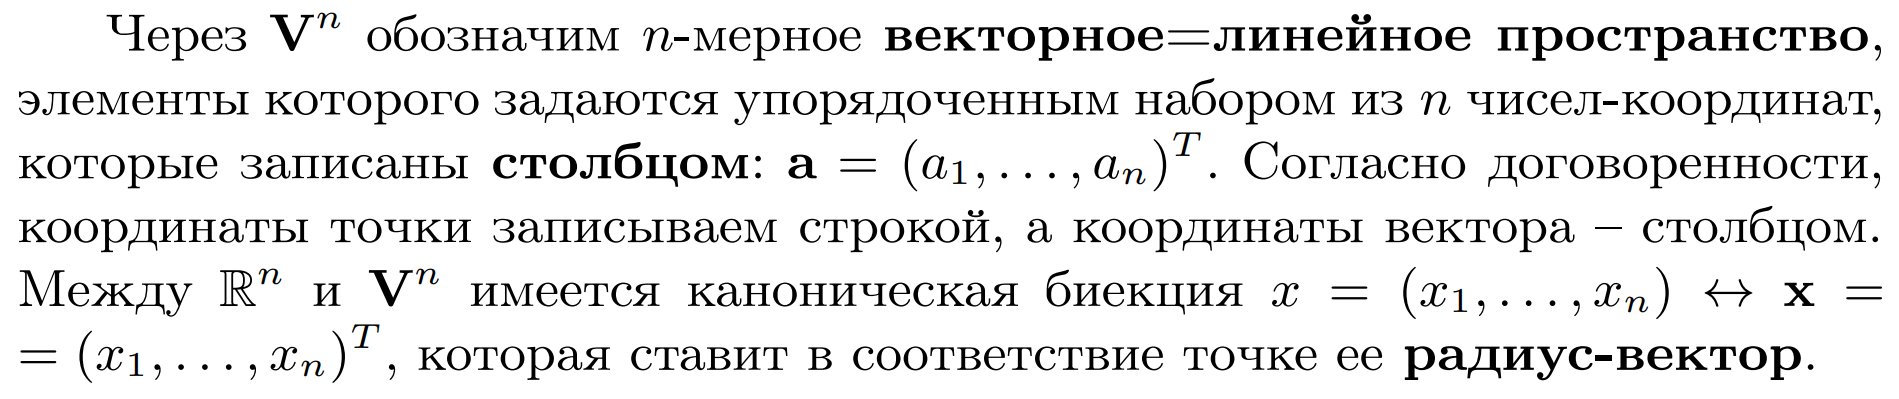
\includegraphics[width=\textwidth]{12.png}
    \vspace{-1cm}
\end{figure}
\begin{figure}[h!]
    \centering
    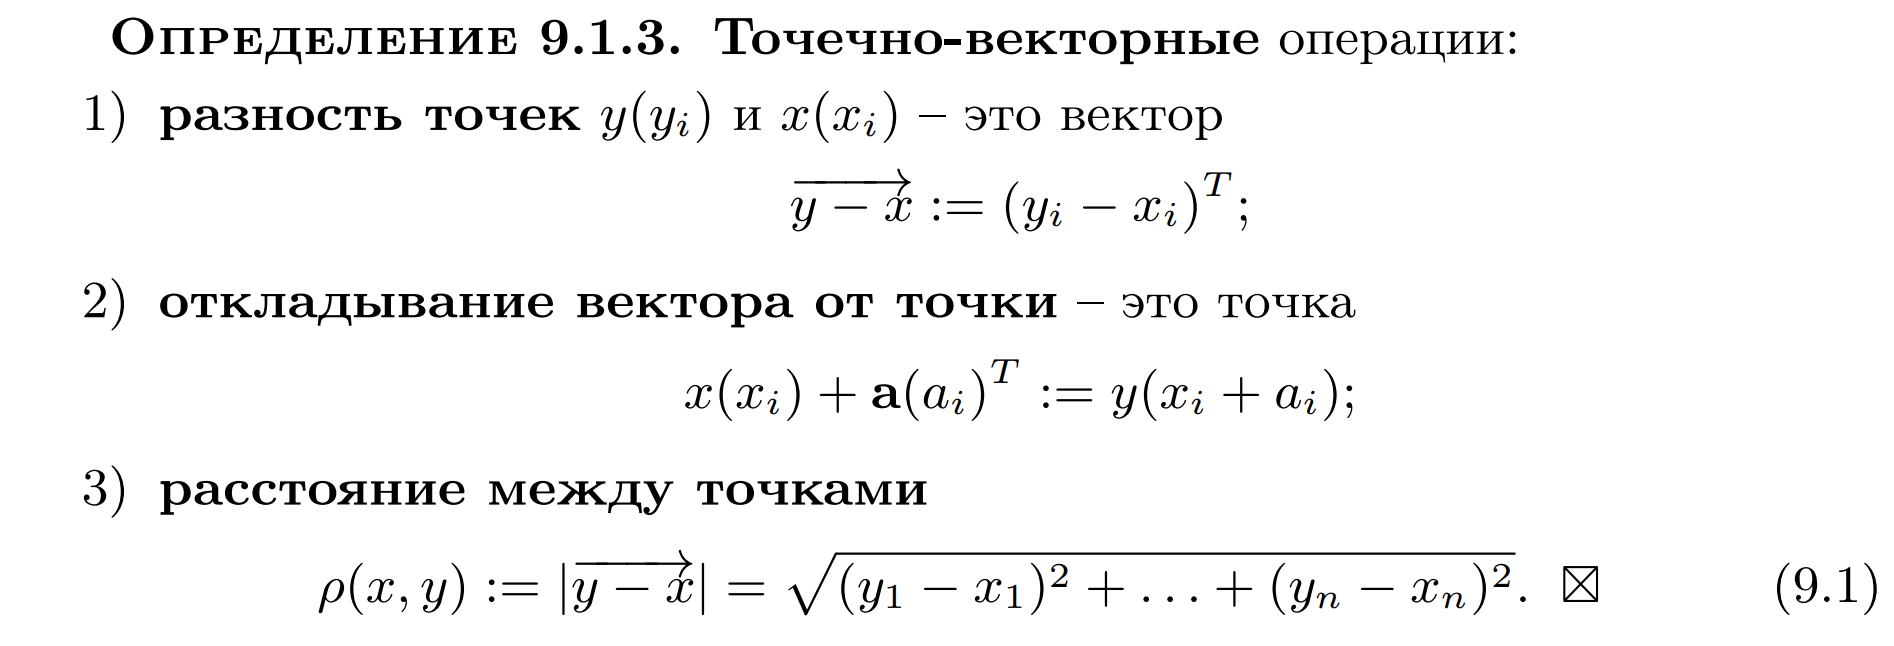
\includegraphics[width=\textwidth]{11.png}
    \vspace{-1cm}
\end{figure}
\begin{figure}[h!]
    \centering
    
\includegraphics[width=\textwidth]{2.png}
    \vspace{-1cm}
\end{figure}
\begin{figure}[h!]
    \centering
    \fbox{
\includegraphics[width=\textwidth]{3.png}}
    \vspace{-1cm}
\end{figure}
\begin{figure}[h!]
    \centering
    \fbox{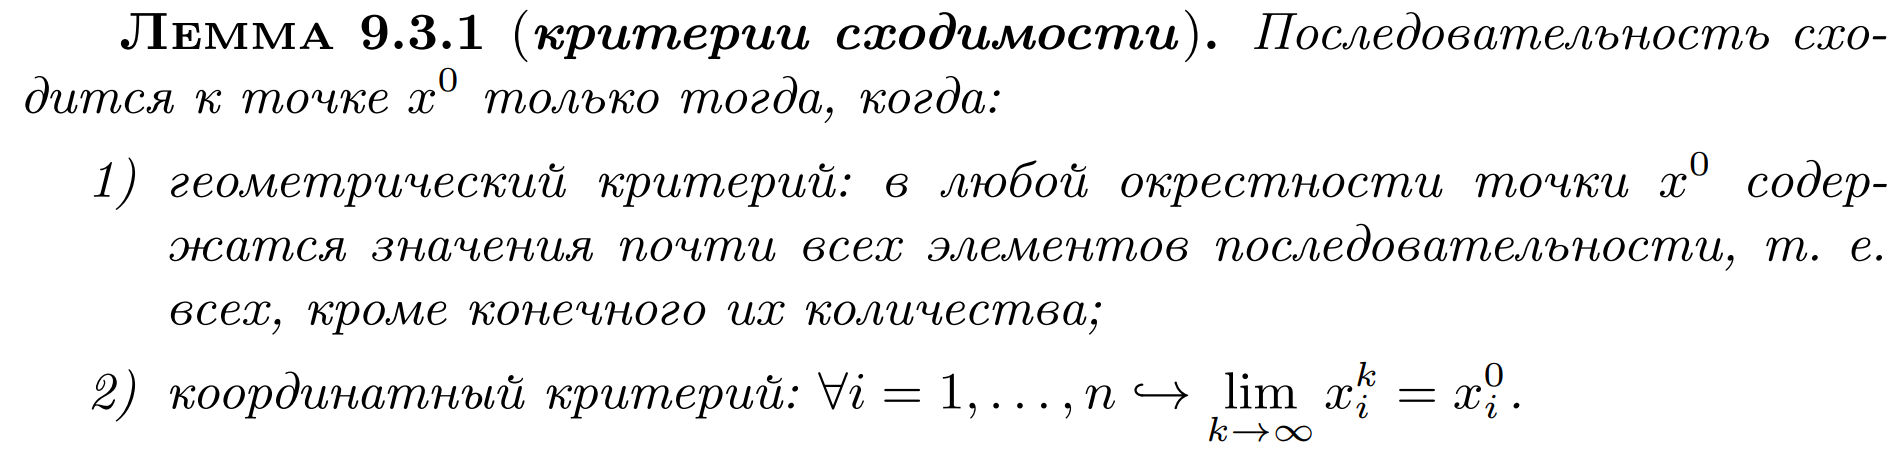
\includegraphics[width=\textwidth]{4.png}}
    \vspace{-1cm}
\end{figure}
\begin{figure}[h!]
    \centering
    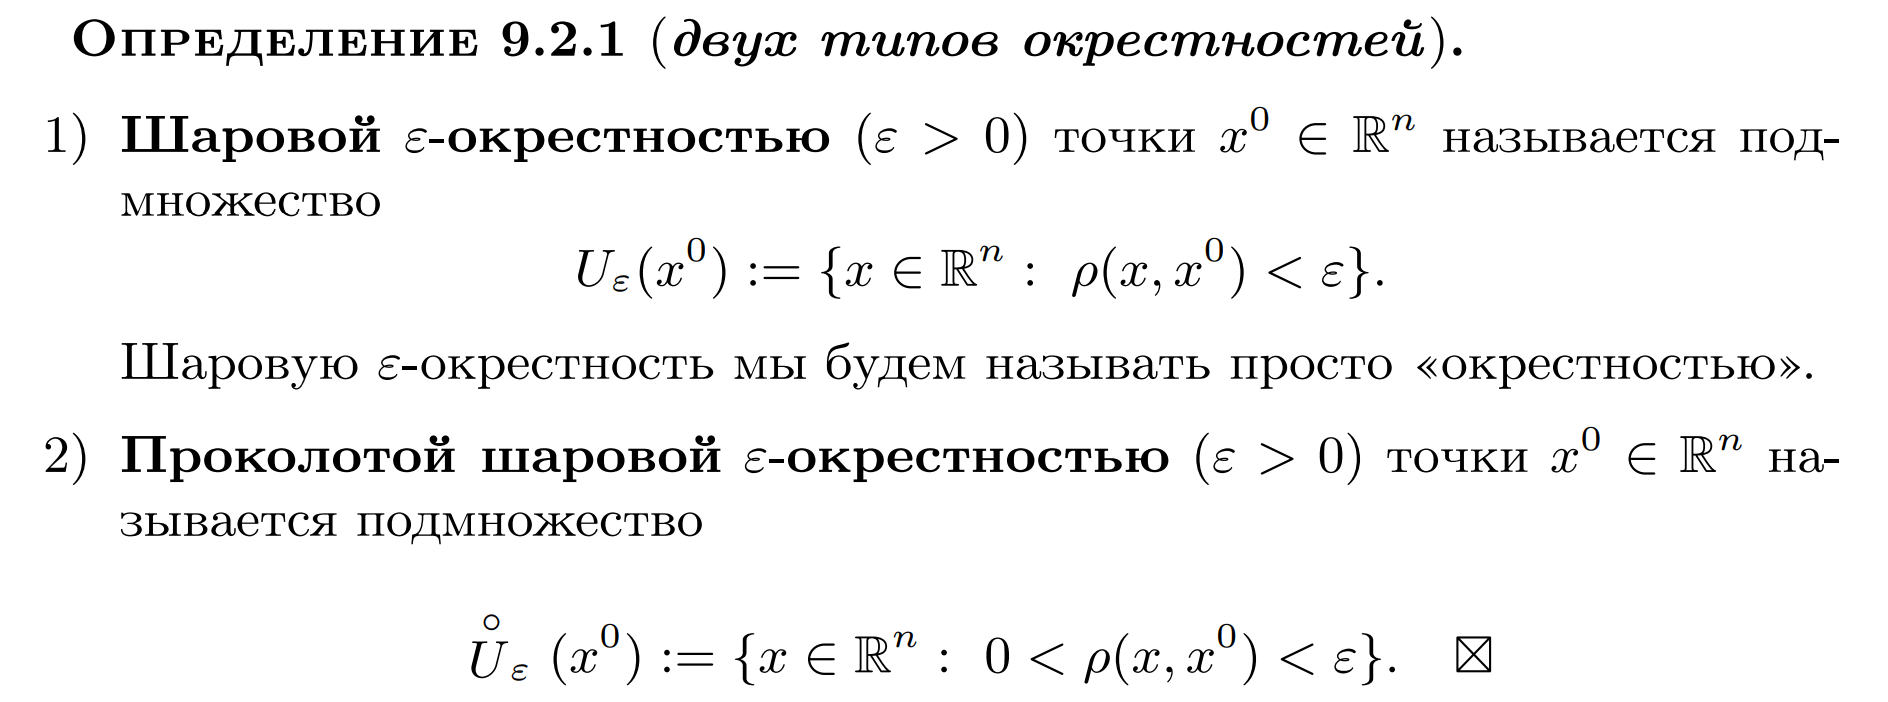
\includegraphics[width=\textwidth]{7.png}
    \vspace{-1cm}
\end{figure}
\newpage
\begin{figure}[h!]
    \centering
    \fbox{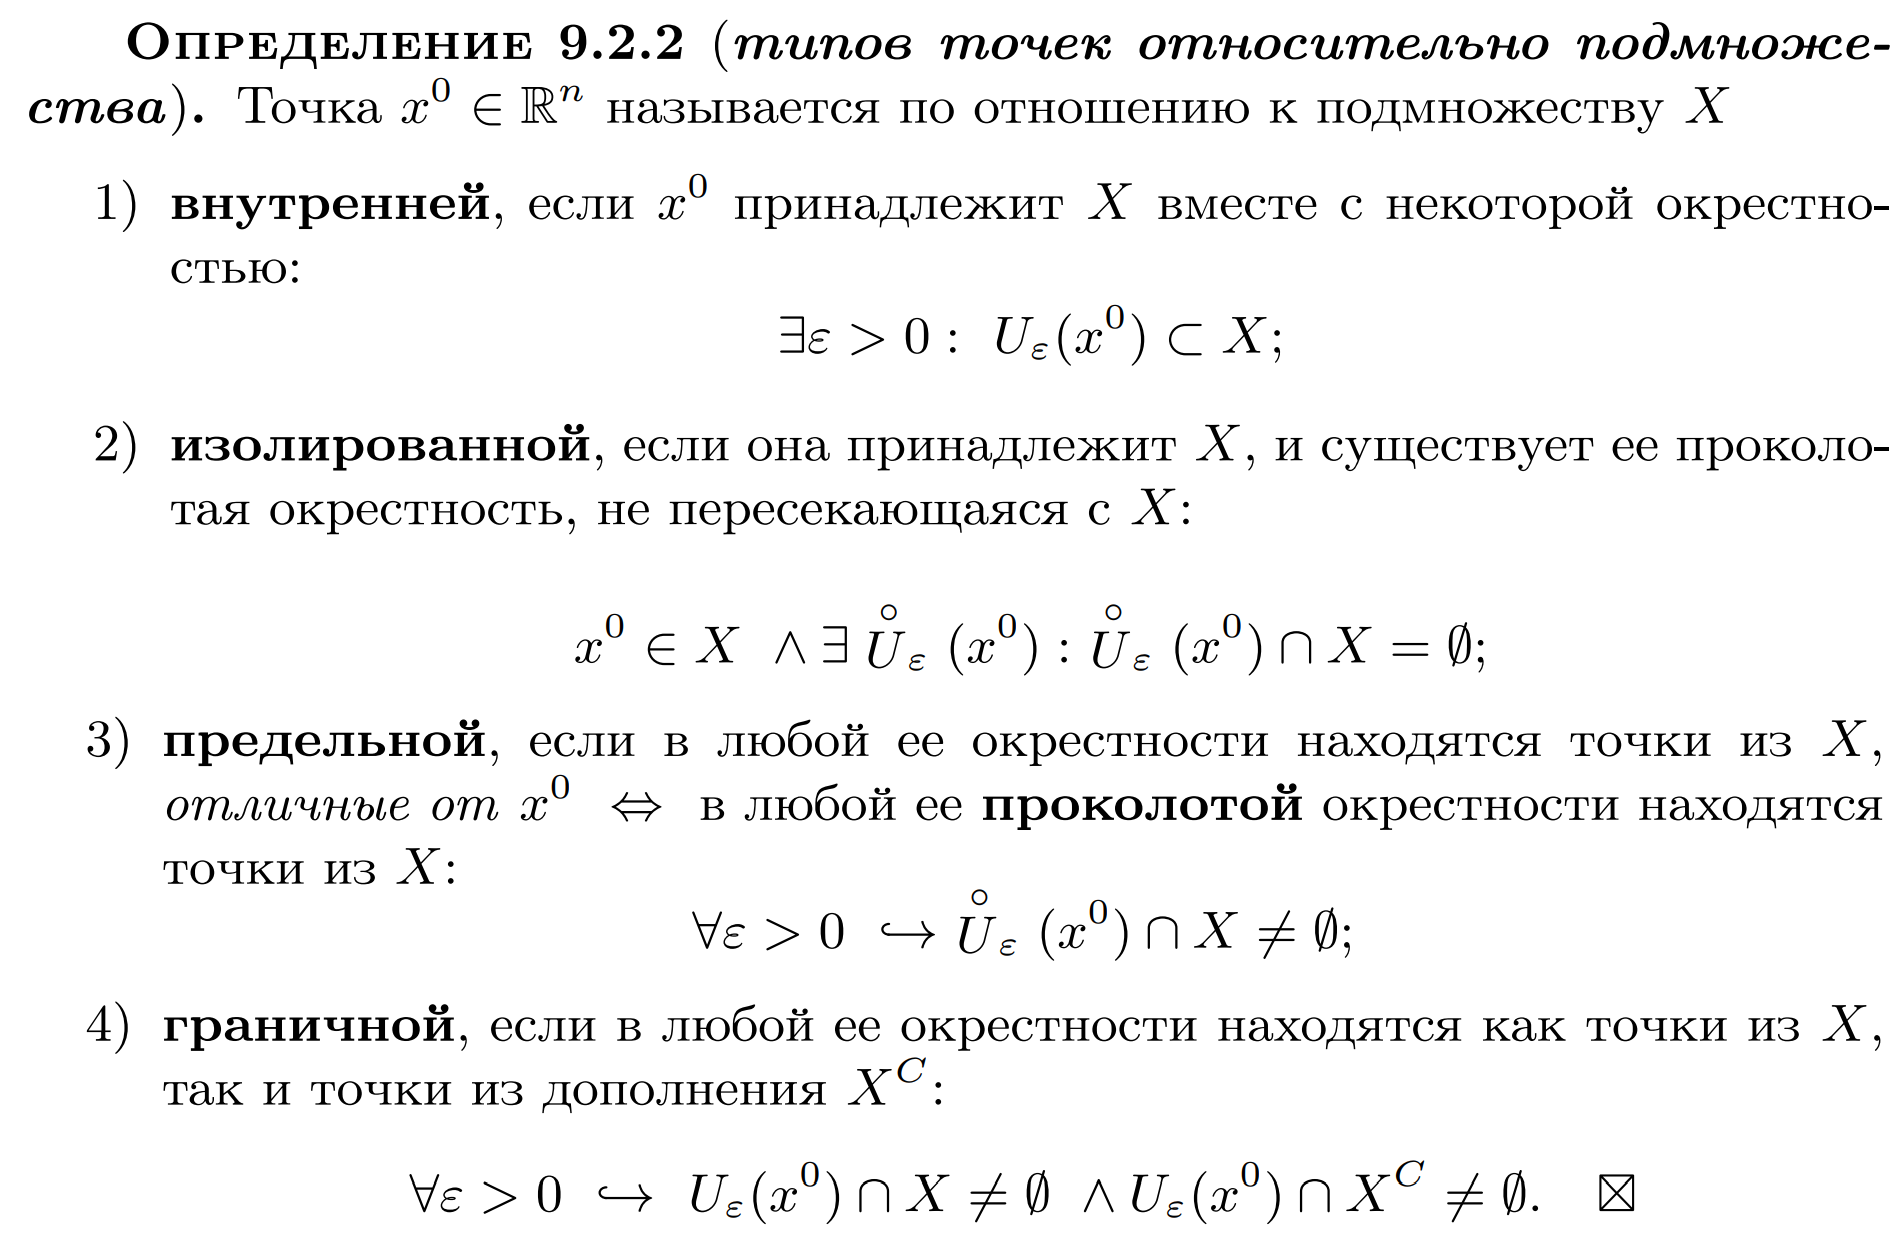
\includegraphics[width=\textwidth]{5.png}}
\end{figure}
Изолированные точки обязательно принадлежат множеству, граничные могут не принадлежать ($(0,1)\cup \{2\}$ и концы $(0,1)$)
\begin{figure}[h!]
    \centering
    
\includegraphics[width=\textwidth]{8.png}
    \vspace{-1cm}
\end{figure}

\bb{Опр} $x_0$ называется точкой прикосновения множества $E$, если в любой её окресности найдутся точки из множества (не проколотой).

Изолированная точка является точкой прикосновения, но не является предельной, любая предельная является изолированной.

\bb{Опр} (эквивалентное) $x^{0}$ -- предельная точка $E$, если $\exists x^{m} \to x^{(0)}, x^{m}\neq x^{(0)}$.

\begin{figure}[h!]
    \centering
    
\includegraphics[width=\textwidth]{9.png}
\end{figure}

\bb{Опр} Область -- открытое, линейно связное множество.

\bb{Опр} $E$ -- линейно связное множество, если $\forall x_1, x_2 \in E$ можем соединить кривойБ принадлежащей $E$

\bb{Опр} Компакт -- ограниченное, замкнутое множество.

\bb{Опр} $E$ -- ограничено, если $\exists U_\varepsilon(0) : E\subset U_\varepsilon(0)$

\begin{figure}[h!]
    \centering
    \fbox{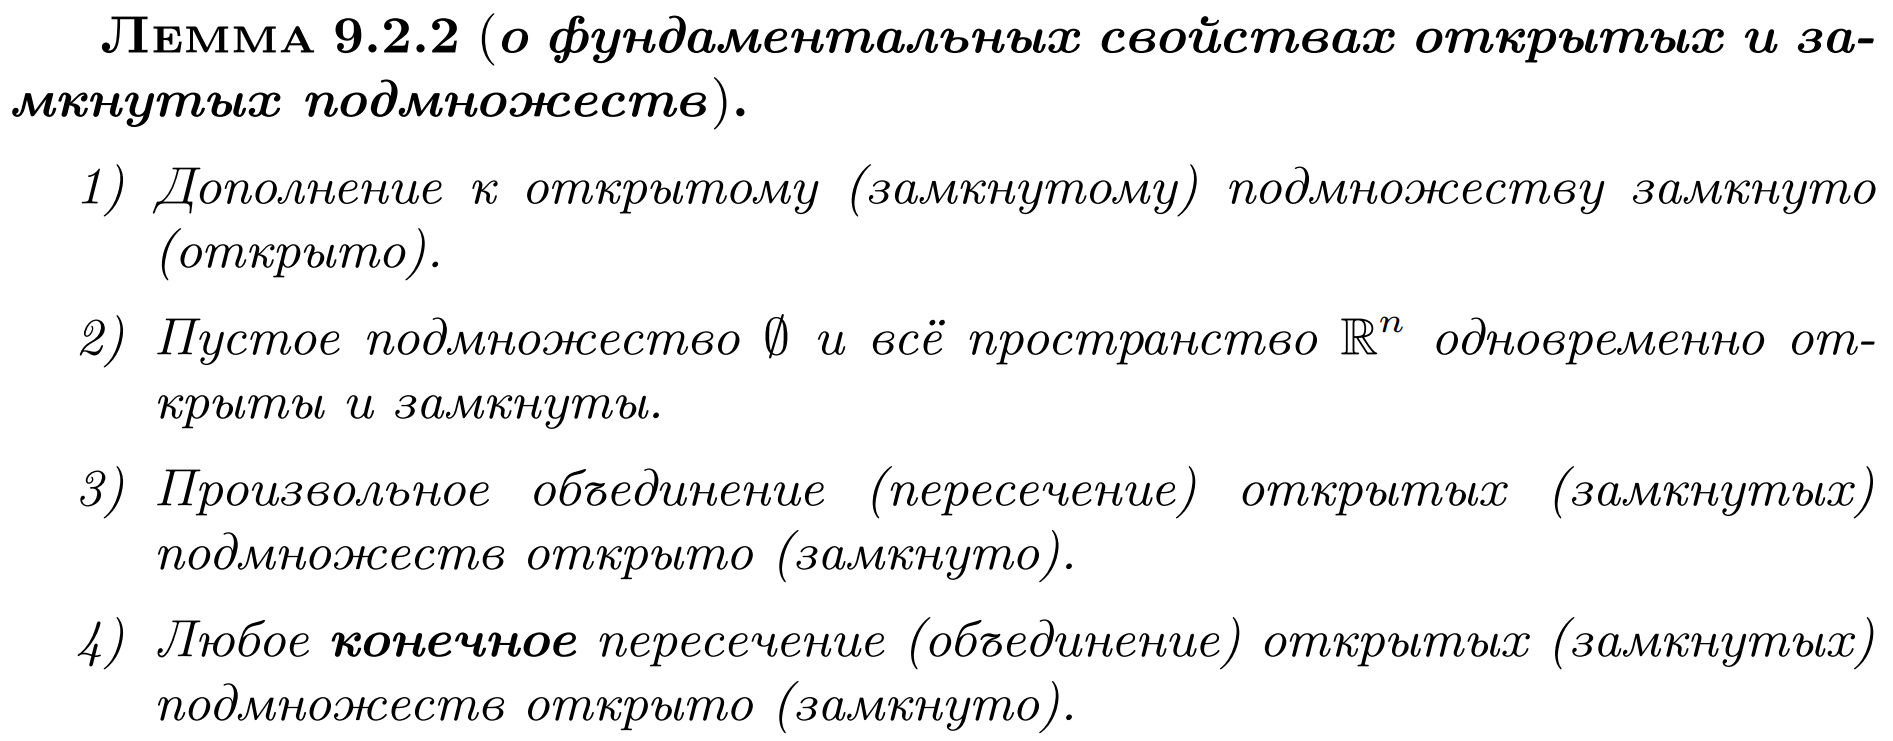
\includegraphics[width=\textwidth]{10.png}}
    \vspace{-1cm}
\end{figure}
\begin{figure}[h!]
    \centering
    \fbox{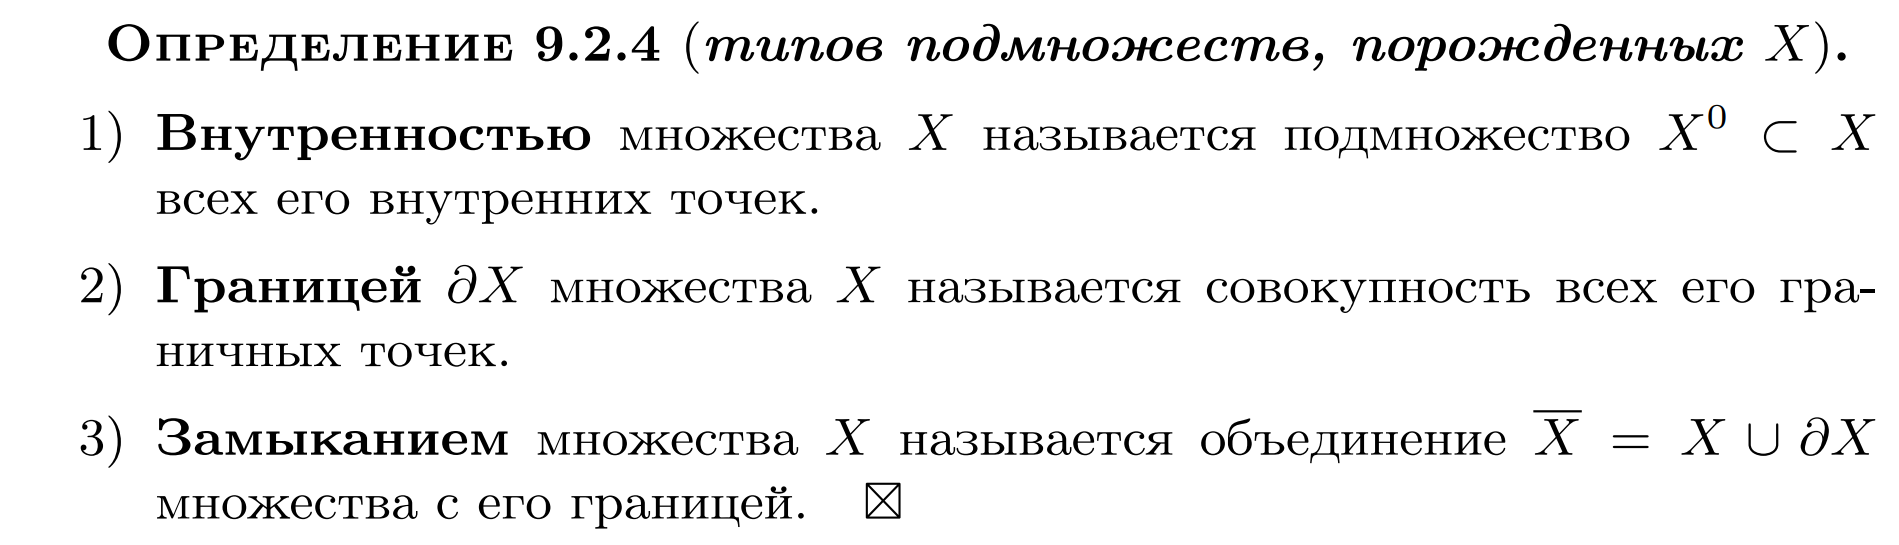
\includegraphics[width=\textwidth]{13.png}}
    \vspace{-1cm}
\end{figure}
\newpage\noindent
\textbf{Предел числовой функции нескольких переменных. Предел функции по множеству. Пределы по направлениям. Непрерывность функции нескольких переменных в точке и по множеству. Непрерывность сложной функции. Свойства функций, непрерывных на компакте — ограниченность, достижимость (точных) нижней и верхней граней, равномерная непрерывность. Теорема о промежуточных значениях функции, непрерывной в области.}
\begin{figure}[h!]
    \centering
    
\includegraphics[width=\textwidth]{14.png}
    \vspace{-1cm}
\end{figure}
\begin{figure}[h!]
    \centering
    \fbox{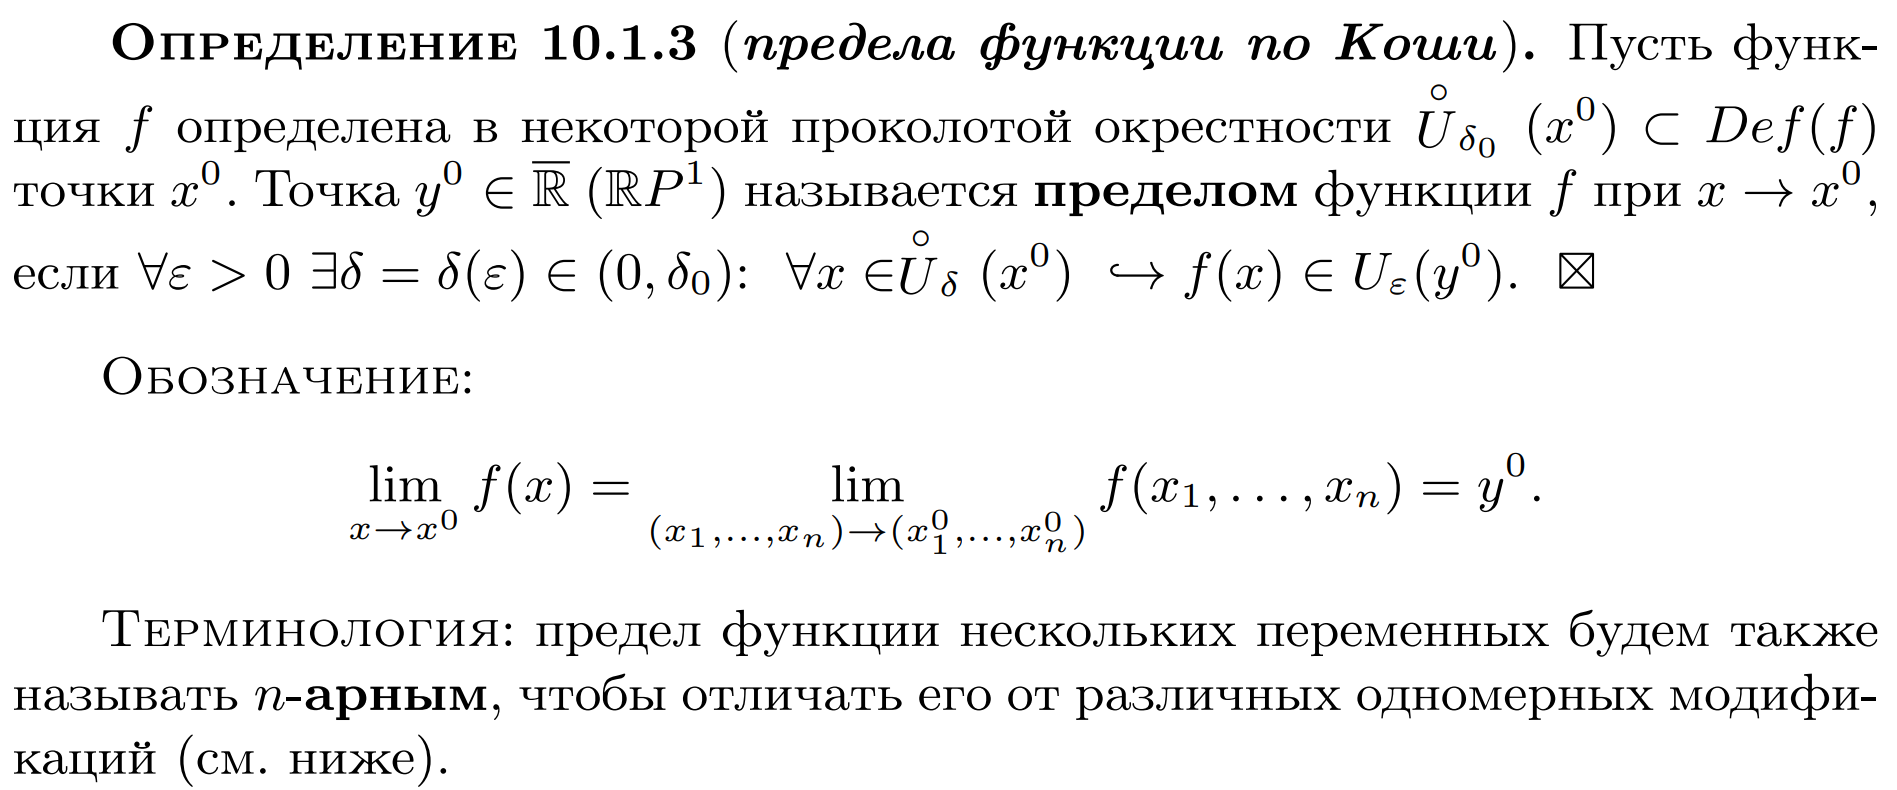
\includegraphics[width=\textwidth]{15.png}}
    \vspace{-1cm}
\end{figure}
\begin{figure}[h!]
    \centering
    \fbox{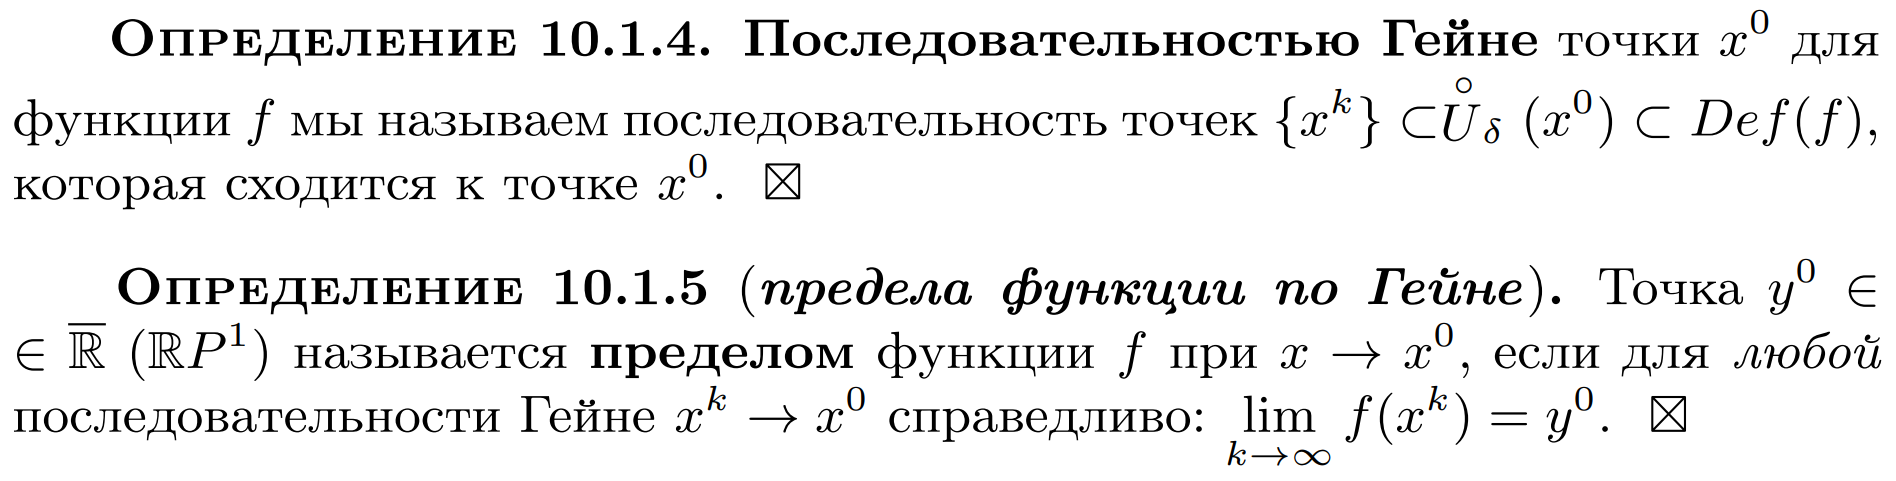
\includegraphics[width=\textwidth]{16.png}}
    \vspace{-1cm}
\end{figure}
\newpage
\begin{figure}[h!]
    \centering
    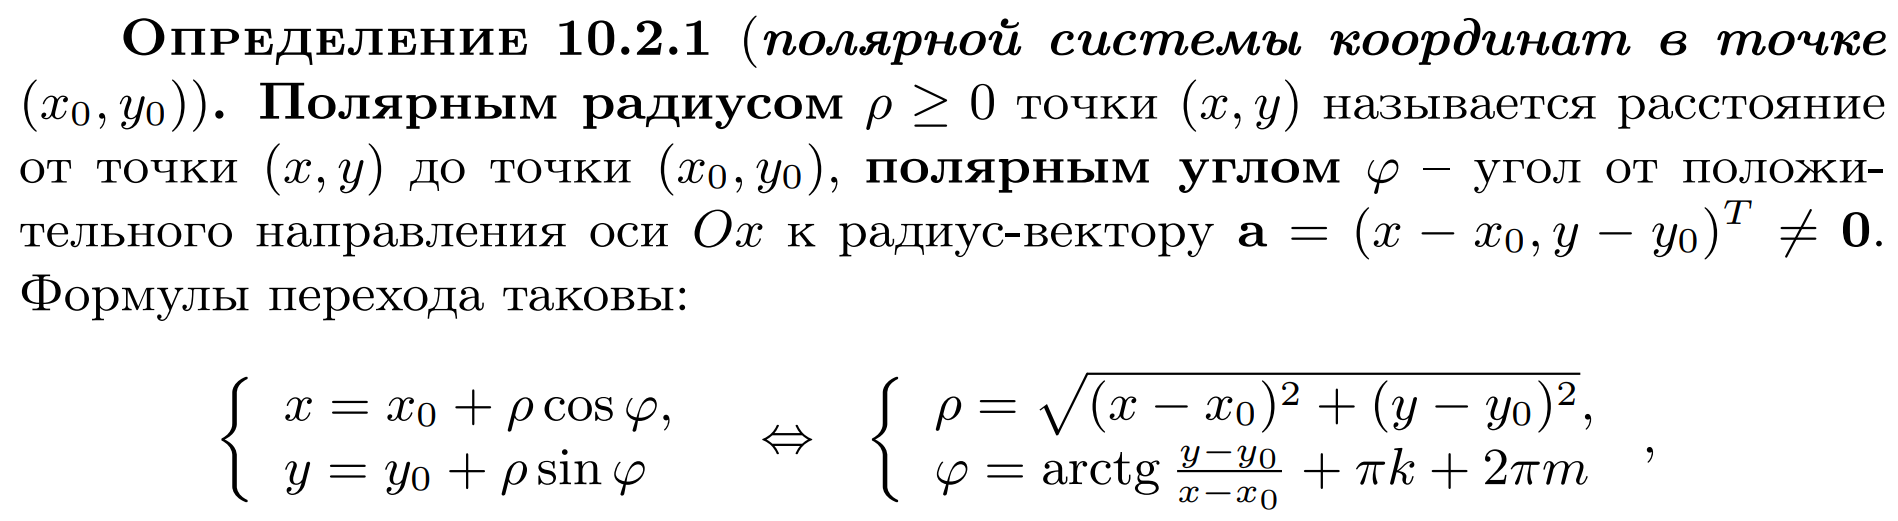
\includegraphics[width=\textwidth]{17.png}
    \vspace{-1cm}
\end{figure}
\begin{figure}[h!]
    \centering
    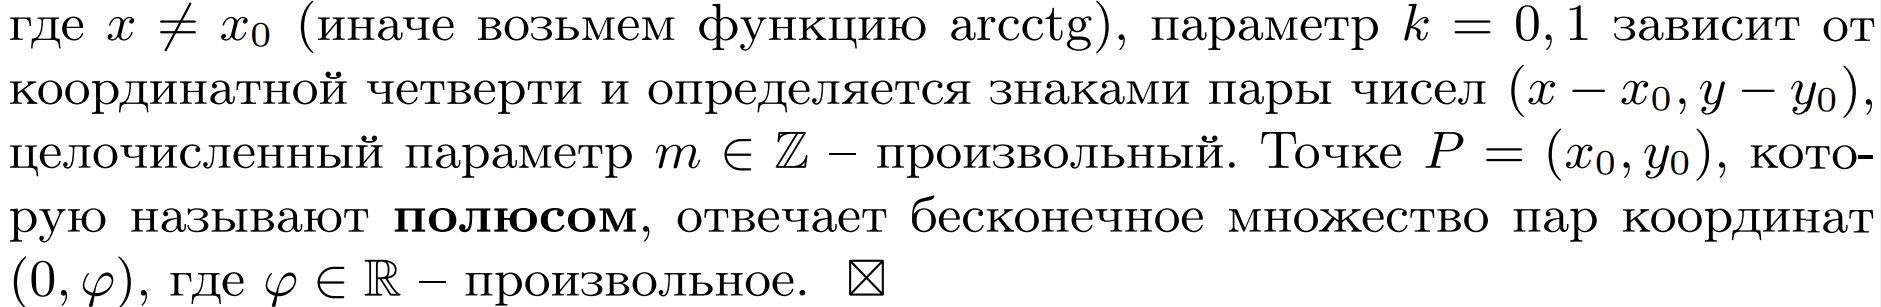
\includegraphics[width=\textwidth]{18.png}
    \vspace{-1cm}
\end{figure}
\begin{figure}[h!]
    \centering
    \fbox{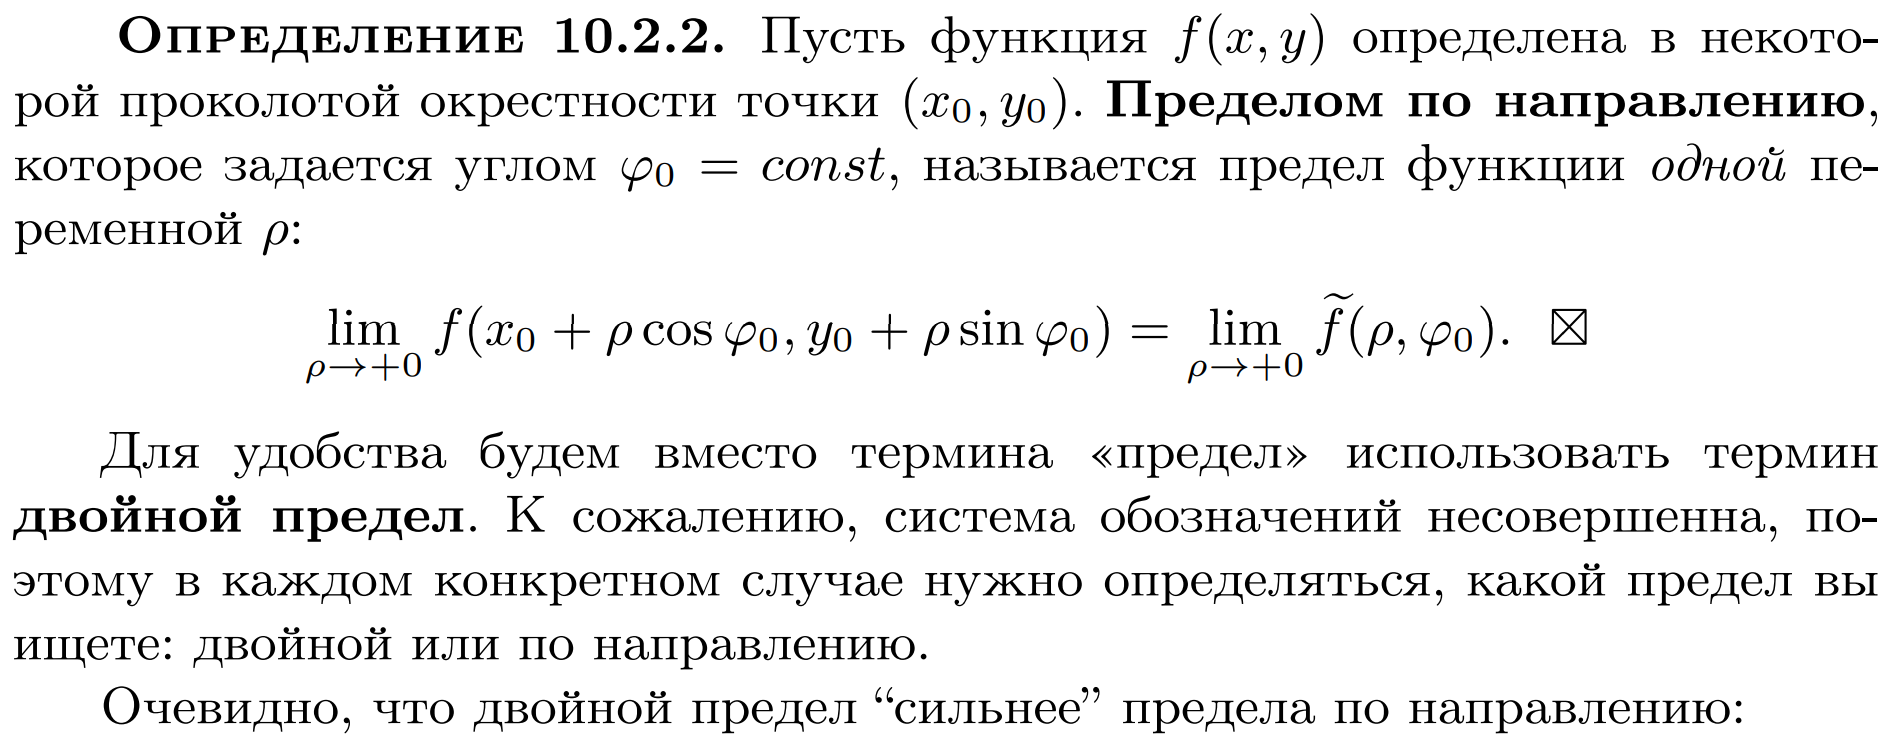
\includegraphics[width=\textwidth]{19.png}}
    \vspace{-1cm}
\end{figure}
\begin{figure}[h!]
    \centering
    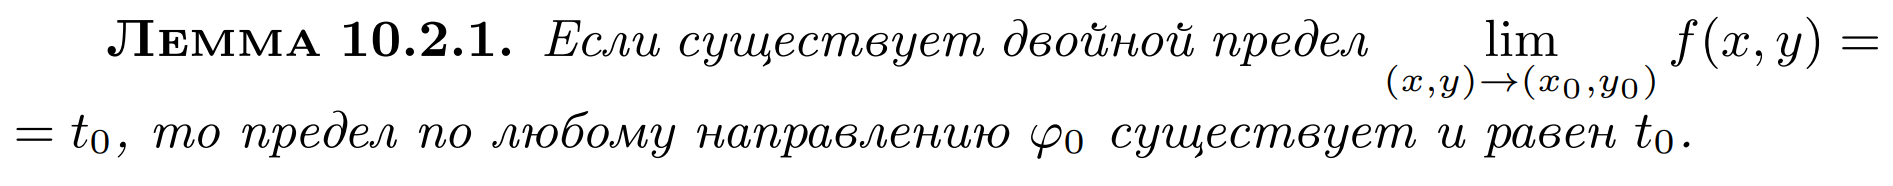
\includegraphics[width=\textwidth]{20.png}
    \vspace{-1cm}
\end{figure}
\begin{figure}[h!]
    \centering
    \fbox{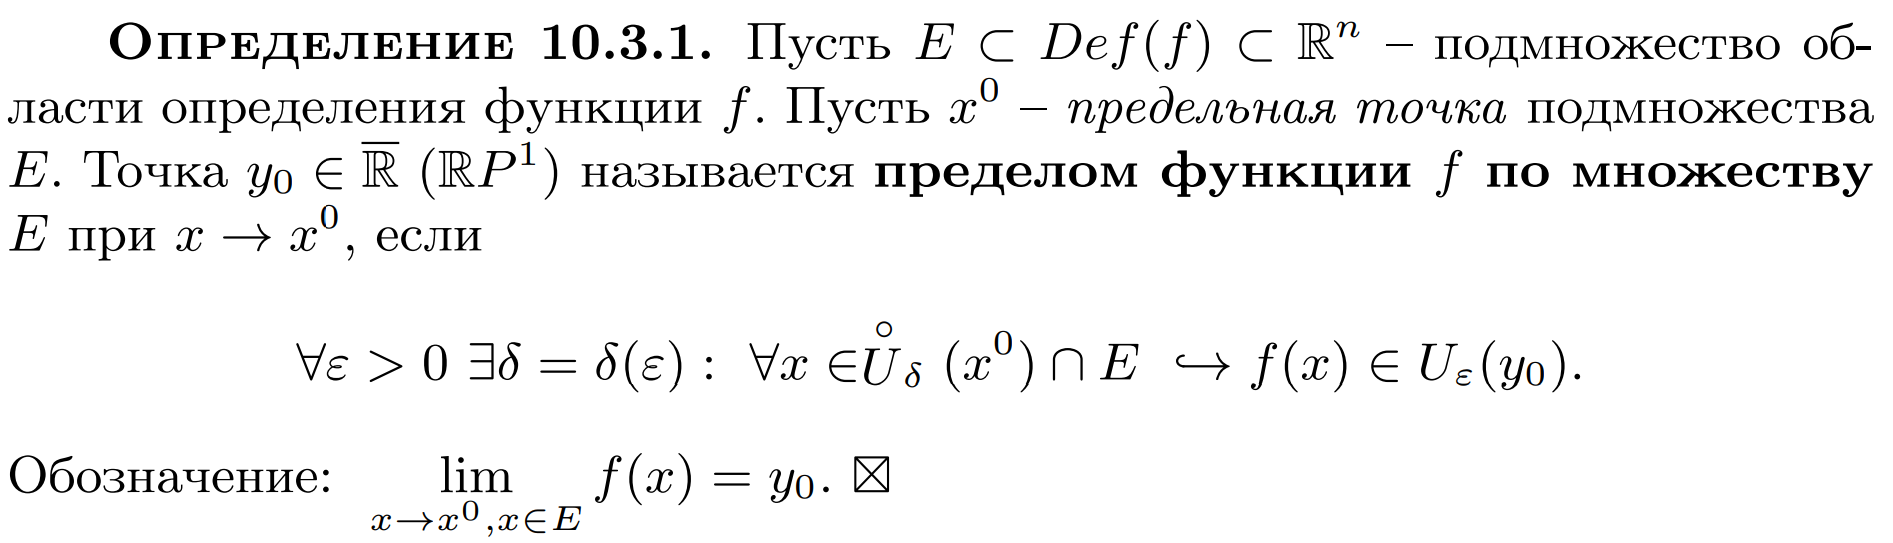
\includegraphics[width=\textwidth]{21.png}}
\end{figure}
Например, односторонние пределы функции одной переменной или предел по направлению функции нескольких переменных.
\newpage
\begin{figure}[h!]
    \centering
    \fbox{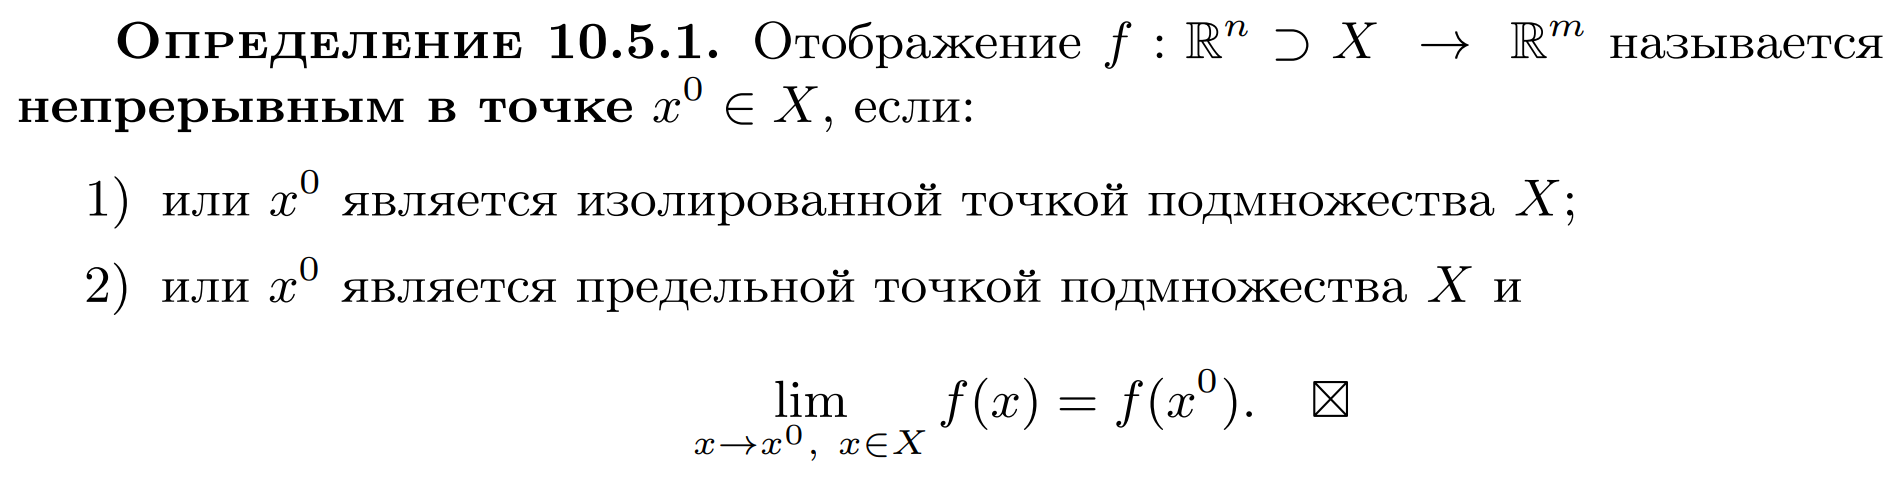
\includegraphics[width=\textwidth]{22.png}}
    \vspace{-1cm}
\end{figure}
\begin{figure}[h!]
    \centering
    
\includegraphics[width=\textwidth]{23.png}
    \vspace{-1cm}
\end{figure}
\begin{figure}[h!]
    \centering
    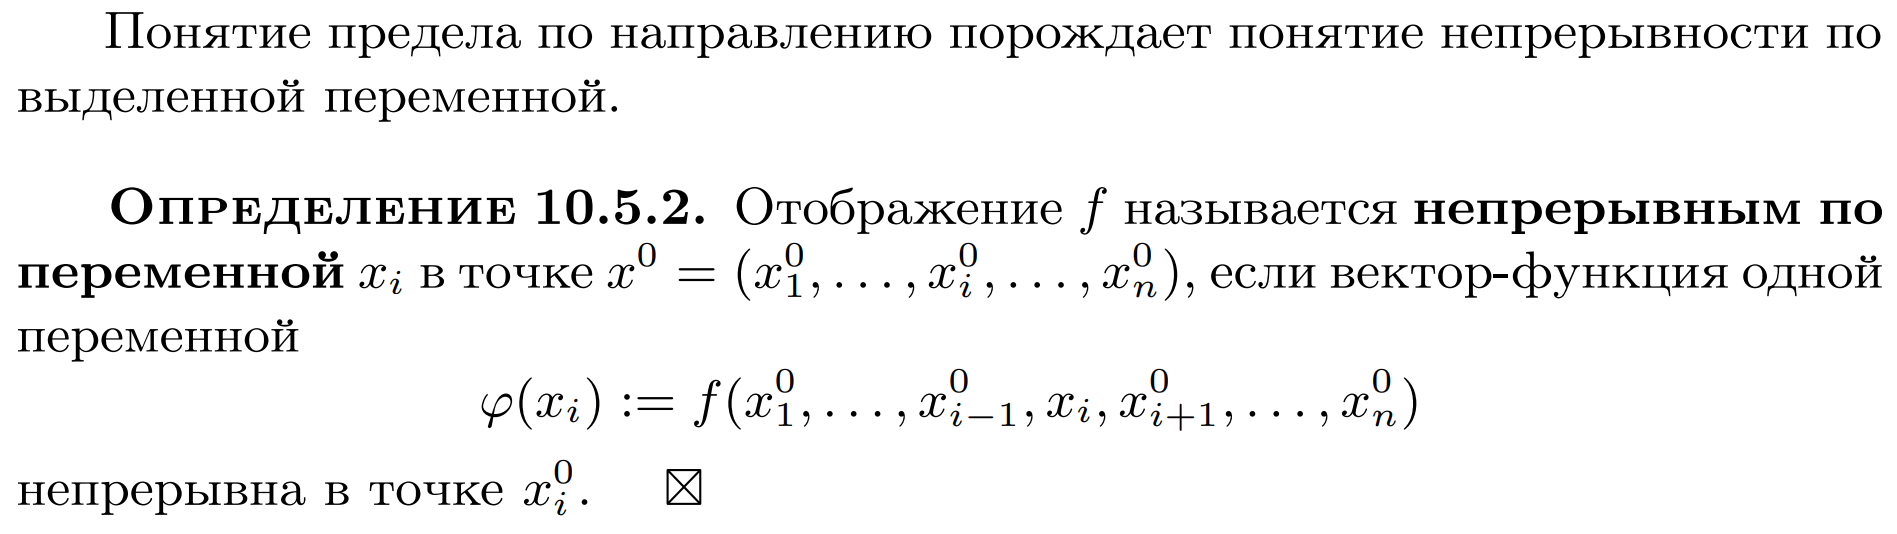
\includegraphics[width=\textwidth]{24.png}
    \vspace{-1cm}
\end{figure}
\begin{figure}[h!]
    \centering
    
\includegraphics[width=\textwidth]{25.png}
    \vspace{-1cm}
\end{figure}
\begin{figure}[h!]
    \centering
    
\includegraphics[width=\textwidth]{26.png}
    \vspace{-1cm}
\end{figure}
\begin{figure}[h!]
    \centering
    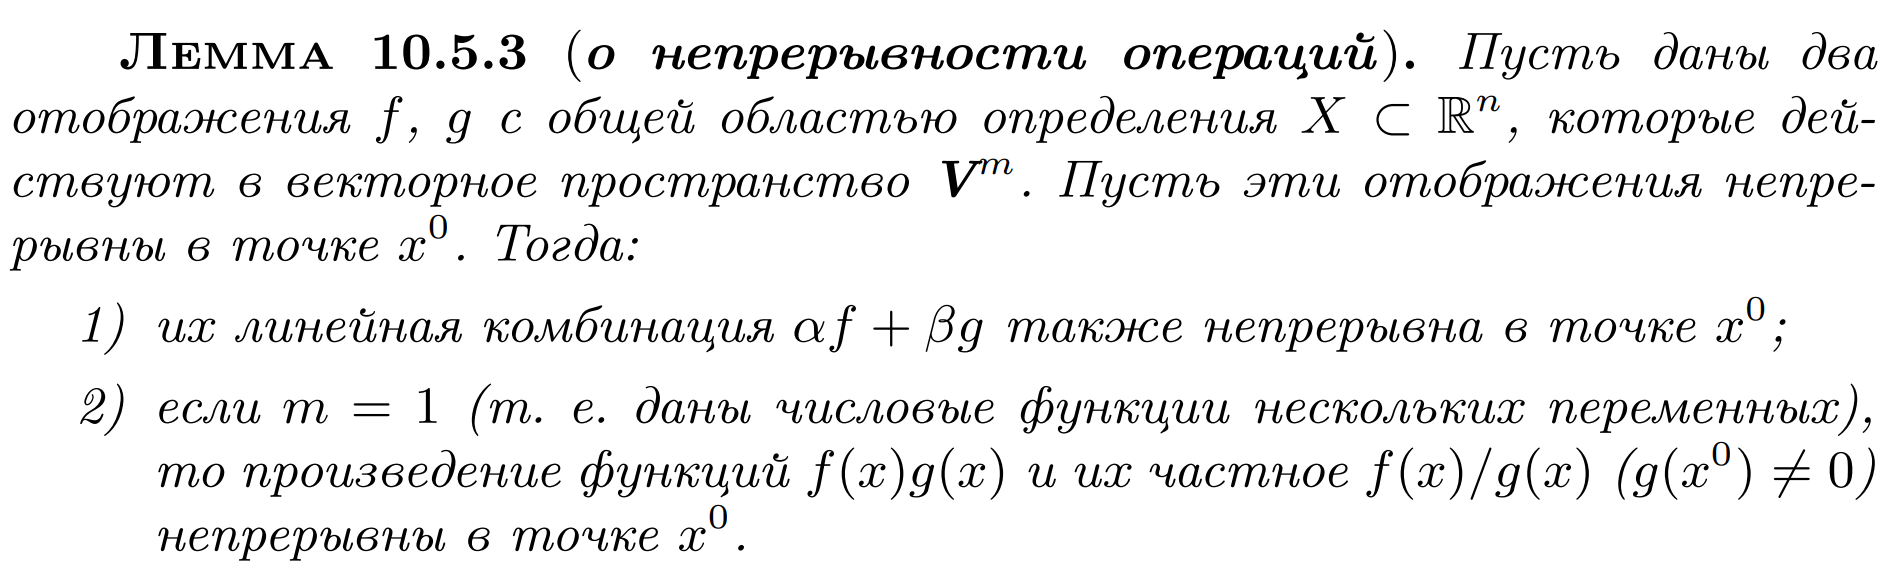
\includegraphics[width=\textwidth]{27.png}
    \vspace{-1cm}
\end{figure}
\newpage
\begin{figure}[h!]
    \centering
    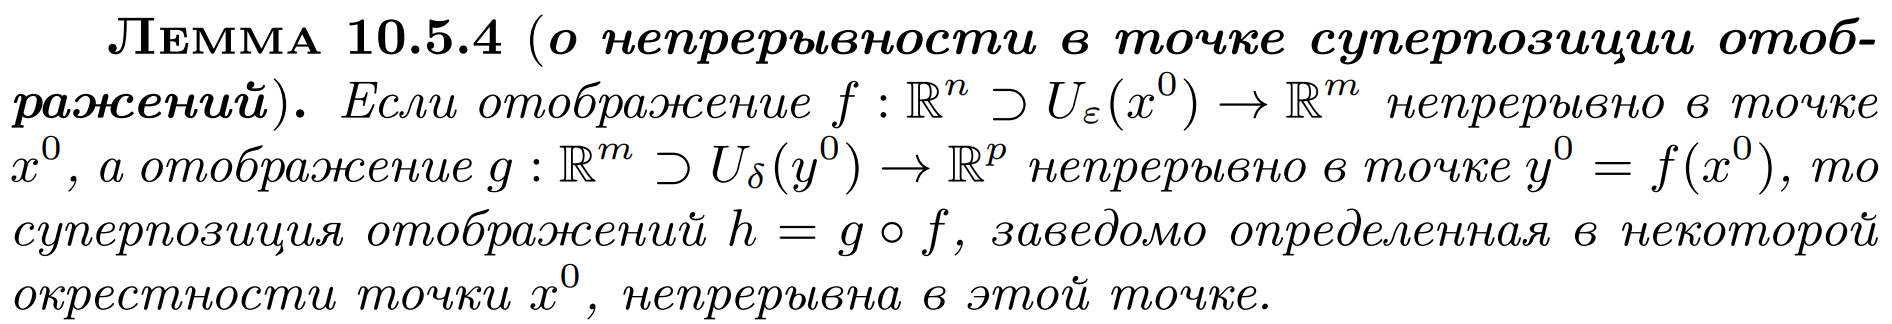
\includegraphics[width=\textwidth]{28.png}
    \vspace{-1cm}
\end{figure}
\begin{figure}[h!]
    \centering
    \fbox{
\includegraphics[width=\textwidth]{29.png}}
    \vspace{-1cm}
\end{figure}
\begin{figure}[h!]
    \centering
    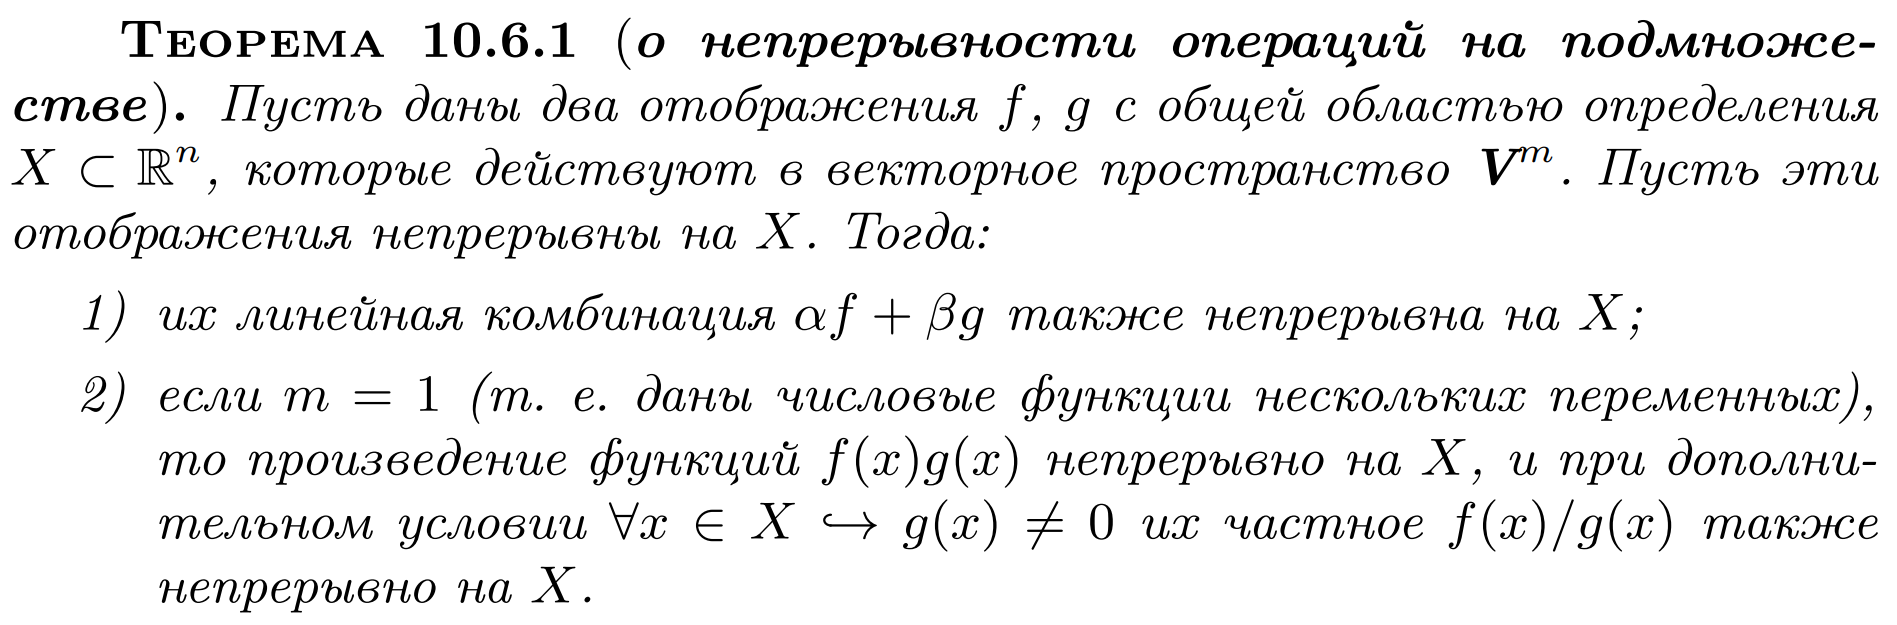
\includegraphics[width=\textwidth]{30.png}
    \vspace{-1cm}
\end{figure}
\begin{figure}[h!]
    \centering
    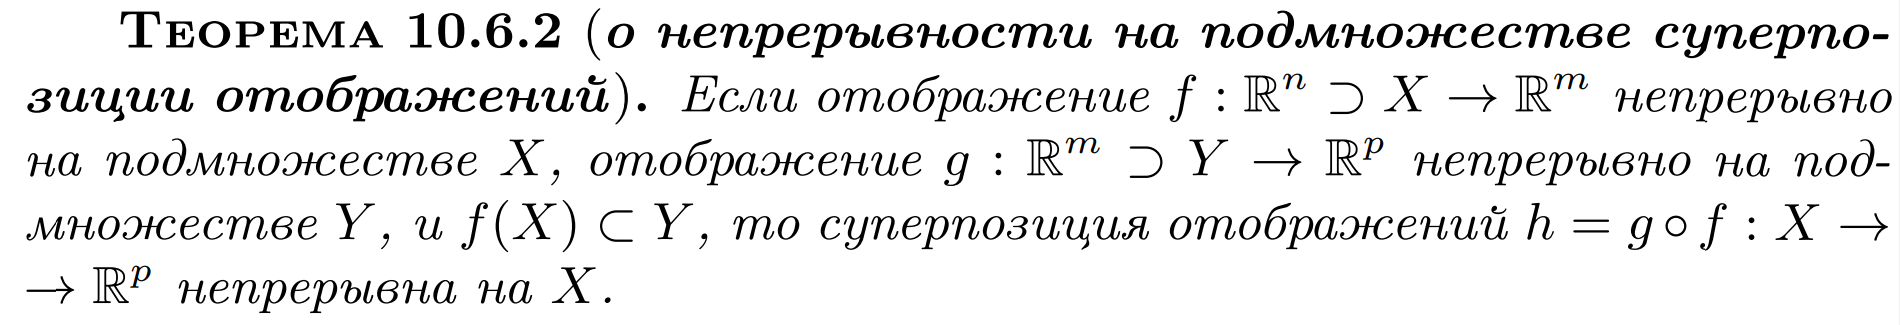
\includegraphics[width=\textwidth]{31.png}
    \vspace{-1cm}
\end{figure}
\begin{figure}[h!]
    \centering
    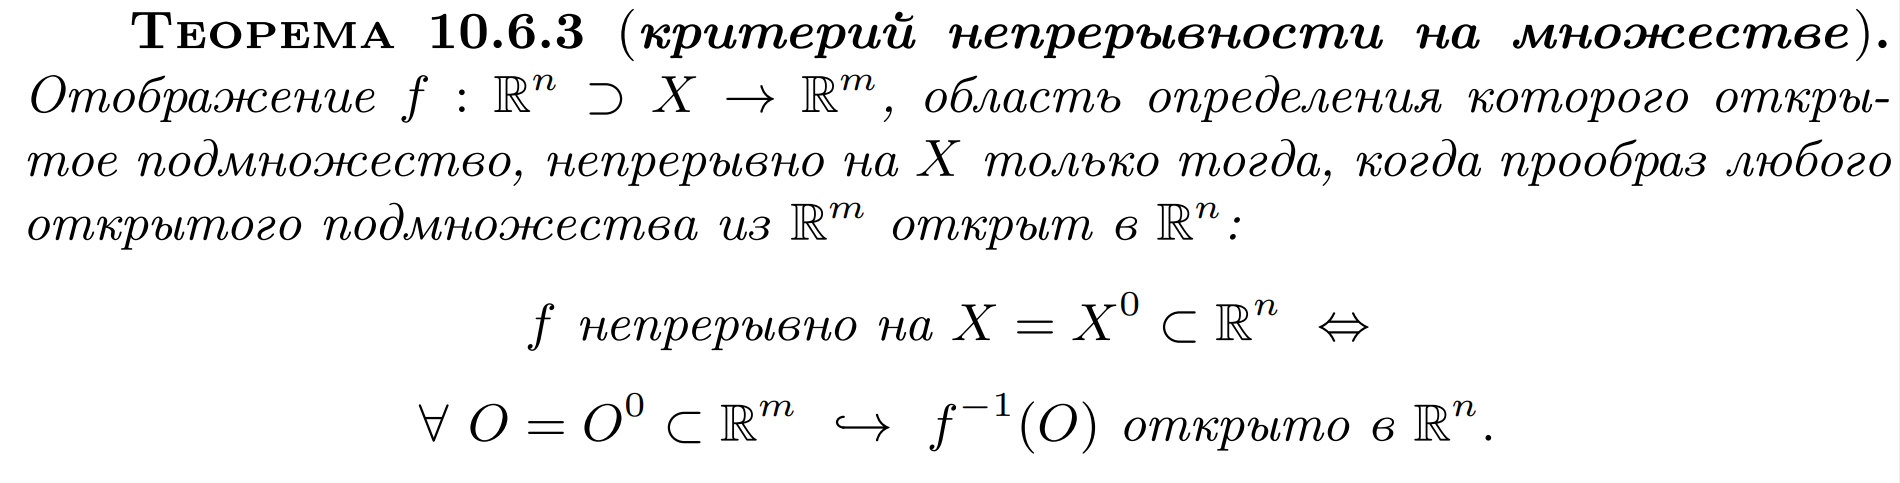
\includegraphics[width=\textwidth]{32.png}
    \vspace{-1cm}
\end{figure}





\end{document}
